\documentclass[11pt, oneside, a4paper]{article}
\setcounter{secnumdepth}{3}
\setcounter{tocdepth}{3}

% Packages
\usepackage{amsmath}
\usepackage{amssymb}
\usepackage[linesnumbered,ruled,vlined]{algorithm2e}
\usepackage[english]{babel}
\usepackage[margin=5pt,labelfont=bf,format=hang,font=small]{caption}
\usepackage{csquotes}
\usepackage{framed}
\usepackage{geometry}
\geometry{a4paper, top=1in, left=1in, right=1in, bottom=1in, headsep=10mm, footskip=20mm}
\usepackage{mathtools}
\usepackage{graphicx}
\usepackage{booktabs}
\usepackage{setspace}
\onehalfspacing
\usepackage{tikz}
\usetikzlibrary{calc, positioning, arrows.meta, fit, backgrounds, decorations.pathreplacing}
\usepackage[hyphens]{url}
\usepackage[
  pdftitle={Exploiting Monotonicity in the Q-Function for DRAUSP via Reinforcement Learning},
  pdfauthor={PDF Autor},
  pdfsubject={Projektbericht}
]{hyperref}

\usepackage{fancyhdr}
\pagestyle{fancy}
\fancyhf{}
\rhead{\small Max Mustermann}
\lhead{\small DRAUSP mit Reinforcement Learning}
\cfoot{\small Page \thepage}

% Literaturverzeichnis
\usepackage[
  backend=biber,
  citestyle=apa,
  style=apa,
  sorting=nyt,
  sortcites=true,
  maxcitenames=2,
  isbn=false]
{biblatex}
\addbibresource{mybib.bib}

% Abkürzungsverzeichnis
\usepackage{acro}

\DeclareAcronym{drausp}{
  short=DRAUSP,
  long=Dynamic Request Acceptance and Unsplittable Scheduling Problem,
}
\DeclareAcronym{rl}{
  short=RL,
  long=Reinforcement Learning,
}
\DeclareAcronym{mdp}{
  short=MDP,
  long=Markov Decision Process,
}
\DeclareAcronym{dqn}{
  short=DQN,
  long=Deep Q-Network,
}

\allowdisplaybreaks

\begin{document}

% Titelseite & Verzeichnisse

\newcommand{\maketitlepage}[7]{
\begin{titlepage}

\begin{center} % zentrieren

  \begin{figure}[ht]
    \centering
    
\includegraphics[width=0.75\linewidth]{grafiken/rptu_logo}
  \end{figure}
  \textbf{\large Wirtschaftswissenschaften \\
  \normalsize Fachgebiet Wirtschaftsinformatik \& Operations Research}\\
  Prof. Dr. Oliver Wendt \\
  \url{http://bisor.wiwi.uni-kl.de/}

  \vfill

  \begin{framed}
    \begin{center}
      \textbf{#1\\}
      \bigskip
      \textsc{{\Large #2}}
    \end{center}
  \end{framed}

  \vfill

  \begin{tabular*}{0.62\textwidth}{r@{\extracolsep{\fill}}l}
   \\
    Betreuer: \quad \qquad & Konstantin Kloster, M.\ Sc. \\
    \\
    Verfasser: \quad \qquad & \textbf{#3}\\
    \quad \qquad & \textsc{#4@rhrk.uni-kl.de}\\
    \quad \qquad &  Matrikel-\textnumero: #5\\
    \quad \qquad & Studiengang: #6\\
    \\
    Eingereicht am: \quad \qquad & #7\\
    \\
  \end{tabular*}
  \vfill
\end{center}

\end{titlepage}
}
\maketitlepage{Projektbericht}{Exploiting Monotonicity in the Q-Function for DRAUSP via Reinforcement Learning}{Max Mustermann, B.\ Sc.}{rhrkacnt}{123456}{WI-ET}{01.01.2026}

\section*{Abstract}
\thispagestyle{empty}
The Dynamic Request Acceptance and Unsplittable Scheduling Problem (DRAUSP) requires an online decision maker to accept or reject incoming requests and, if accepted, to schedule them as contiguous blocks across multiple capacity-limited resources, so as to maximize cumulated revenue over a finite horizon. \\
While exact stochastic dynamic programming solves DRAUSP optimally, it becomes computationally intractable as the number of resources and requests grows. This report formulates DRAUSP as a finite-horizon Markov Decision Process and learns an acceptance-and-scheduling policy via value-based deep reinforcement learning. A standard Deep Q-Network (DQN) with action masking and a reject-biased exploration scheme serves as the baseline. Since the problem exhibits domain structure that a generic network is not guaranteed to respect -- e.g., more remaining capacity or a higher-reward request should never yield a lower $Q$-value -- the goal of this work is to develop a Lattice-DQN that enforces this structure using a Deep Lattice Network architecture. We test the monotonicity of the learned $Q$-functions and compare the performance of both agents on a set of benchmark instances of \textcite{drausp_lion18} under a parameter-matched comparison. The Standard-DQN reaches $90$--$100\%$ of the optimal objective value on most instances and, without any structural constraints, already learns near-perfect monotonicity in most state components. The Lattice-DQN satisfies all monotonicity relations exactly by construction, but its more constrained function class leads to slower convergence and lower reward on harder, longer-horizon instances. These results suggest that structural monotonicity constraints guarantee reliable, interpretable $Q$-functions at the cost of reduced policy flexibility, motivating hybrid architectures as a direction for future work.

\clearpage


\pagenumbering{Roman}
\tableofcontents
\cleardoublepage
\phantomsection
\addcontentsline{toc}{section}{List of Abbreviations}
\printacronyms[name=List of Abbreviations]
\clearpage
\phantomsection
\addcontentsline{toc}{section}{List of Figures}
\listoffigures
\clearpage
\phantomsection
\addcontentsline{toc}{section}{List of Tables}
\listoftables
\clearpage
\pagenumbering{arabic}
\setcounter{page}{1}

% Inhalt
\section{Introduction}
\label{sec:introduction}

TODO: Motivation, Problemstellung und Aufbau des Berichts.

\section{Problem Description: DRAUSP}
\label{sec:drausp}

TODO: Formale Beschreibung des Dynamic Request Admission / Utilization Scheduling Problems (DRAUSP), Notation, Zielfunktion, Restriktionen.

\section{Reinforcement Learning Approach}
\label{sec:rl-approach}

TODO: Belohnungsfunktion, DQN-Agent (Trainingsschleife, Replay-Buffer, Zielnetzwerk, $\epsilon$-greedy).

To use reinforcement learning techniques for modeling the \ac{drausp}, first of all we need to define
a \ac{mdp} that represents the problem. We define a state space,an action space and a transition function: 

\textbf{State space.} A state
\[
  s = (t, \hat C_1, \dots, \hat C_K, r, q_1, \dots, q_K) \in \mathcal{S} \subseteq \mathbb{R}^{2K+2}
\]
consists of the current decision epoch $t \in \{1,\dots,T_d\}$, the remaining capacities
$\hat C_k \in \{0,\dots,C_k^{(0)}\}$ of each resource $k=1,\dots,K$, and the $t$-th request $[r,q]$
currently up for decision, with reward $r \in \mathbb{R}_{\ge 0}$ and (zero-padded) demand vector
$q \in \mathbb{N}_0^K$:
\begin{equation}
  \label{eq:padding}
  q = (\underbrace{q_1, \dots, q_\ell}_{\text{demanded capacities}},\; \underbrace{0, \dots, 0}_{K-\ell \text{ padding}}\,).
\end{equation}
The initial state is $s_1 = (1, C_1^{(0)}, \dots, C_K^{(0)}, r_1, q_1)$.

\textbf{Action space.} $\mathcal{A} = \{0,1,\dots,K\}$: action $a=0$ rejects the current request; action $a \in \{1,\dots,K\}$ accepts it and schedules it starting at slot $a$.
Assume that the current request has length $\ell \in \{1,\dots,K\}$ and demand vector $q = (q_1,\dots,q_\ell,0,\dots,0)$ (zero-padded to length $K$). Then the action $a$ is feasible if and only if 
\begin{itemize}
 \item $a+\ell-1 \le K$, we do not exceed the maximum length of resources
 \item $\hat C_{a+i-1} \ge q_i$ for all $i=1,\dots,\ell$, the capacity of all affected slots is sufficient to accept the request
\end{itemize} 
Note that for a given state not all actions are feasible: We define the feasible action set $\mathcal{A}_s^{\text{valid}} \subseteq \mathcal{A}$ as the set of actions that do not exceed the remaining capacity of any affected slot and do not exceed the horizon $K$.
Nevertheless the set of valid actions $\mathcal{A}_s^{\text{valid}}$ is never empty, since $0 \in \mathcal{A}_s^{\text{valid}}$ for all states $s$.
We will use the set of valid actions later on.

\textbf{Transition function.} $\mathcal{T}: \mathcal{S} \times \mathcal{A} \to \mathcal{S}$
deterministically updates the remaining capacities according to the chosen action, appends the next request
$[r_{t+1}, q_{t+1}]$ drawn from the instance's request sequence, and advances time, $t \mapsto t+1$. 
The new capacities are given by the following equation:
\[
  \hat C_{a+i-1} \;\leftarrow\; \hat C_{a+i-1} - q_i, \qquad i = 1,\dots,\ell.
\]
Note that $\hat{C_k} \geq 0$ for all valid actions $a \in \mathcal{A}_x^{\text{valid}}$ and all $k=1,\dots,K$.

Figure~\ref{fig:state-transition} illustrates the effect of the transition function $\mathcal{T}$ on a concrete example with
$K=5$, request length $\ell=3$, action $a=2$ and applies the update rule.

\begin{figure}[htbp]
  \centering
  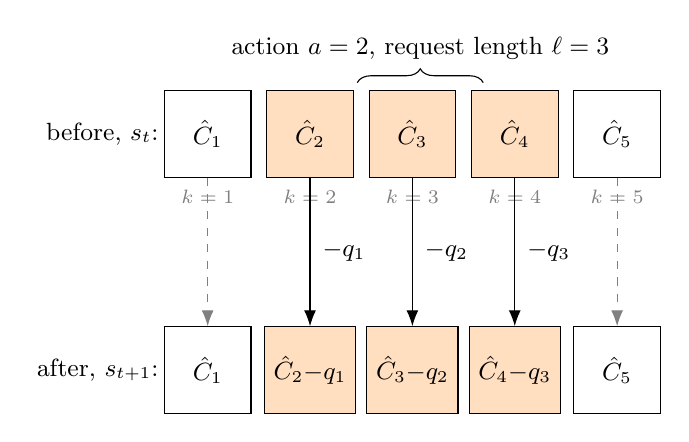
\begin{tikzpicture}[font=\small,
      slot/.style={draw, minimum width=11mm, minimum height=11mm},
      occ/.style ={draw, fill=orange!25, minimum width=11mm, minimum height=11mm},
      >={Latex[length=2mm]}
    ]
    % Before-row: state s at epoch t
    \node[anchor=east] at (-0.5,0)  {before, $s_t$:};
    \node[slot] (b1) at (0,0)   {$\hat C_1$};
    \node[occ]  (b2) at (1.3,0) {$\hat C_2$};
    \node[occ]  (b3) at (2.6,0) {$\hat C_3$};
    \node[occ]  (b4) at (3.9,0) {$\hat C_4$};
    \node[slot] (b5) at (5.2,0) {$\hat C_5$};

    \node[below=1pt, gray] at (b1.south) {\scriptsize $k=1$};
    \node[below=1pt, gray] at (b2.south) {\scriptsize $k=2$};
    \node[below=1pt, gray] at (b3.south) {\scriptsize $k=3$};
    \node[below=1pt, gray] at (b4.south) {\scriptsize $k=4$};
    \node[below=1pt, gray] at (b5.south) {\scriptsize $k=5$};

    \draw[decorate, decoration={brace, amplitude=5pt}] (1.85+0.05,0.65) -- (3.55-0.05,0.65)
      node[midway, above=5pt] {action $a=2$, request length $\ell=3$};

    % After-row: state s_{t+1} after applying T
    \node[anchor=east] at (-0.5,-3) {after, $s_{t+1}$:};
    \node[slot] (a1) at (0,-3)   {$\hat C_1$};
    \node[occ]  (a2) at (1.3,-3) {$\hat C_2{-}q_1$};
    \node[occ]  (a3) at (2.6,-3) {$\hat C_3{-}q_2$};
    \node[occ]  (a4) at (3.9,-3) {$\hat C_4{-}q_3$};
    \node[slot] (a5) at (5.2,-3) {$\hat C_5$};

    \draw[->, dashed, gray] (b1) -- (a1);
    \draw[->] (b2) -- node[right, xshift=1pt] {$-q_1$} (a2);
    \draw[->] (b3) -- node[right, xshift=1pt] {$-q_2$} (a3);
    \draw[->] (b4) -- node[right, xshift=1pt] {$-q_3$} (a4);
    \draw[->, dashed, gray] (b5) -- (a5);
  \end{tikzpicture}
  \caption{Effect of the transition function $\mathcal{T}$ ($K=5$ slots, request length $\ell=3$, action $a=2$): the
    remaining capacities of the three occupied slots each decrease by the corresponding entry of
    the demand vector $q$, while the capacities of slots outside the accepted block ($k=1,5$)
    are unaffected.}
  \label{fig:state-transition}
\end{figure}

\textbf{Reward.} The reward function $\mathcal{R}: \mathcal{S} \times \mathcal{A} \to \mathbb{R}$ is defined as follows:
\[
  \mathcal{R}(s,a) =
  \begin{cases}
    r, & \text{if } a \in \mathcal{A}_s^{\text{valid}} \setminus \{0\} \\
    0, & \text{if } a = 0 \\
    -100, & \text{if } a \notin \mathcal{A}_s^{\text{valid}}
  \end{cases}
\]
Selecting an infeasible action, terminates the episode and yields a large negative reward of $-100$ to discourage the agent from taking invalid actions.

\textbf{Objective.} 
Given a MDP the goal is to find a policy $\pi$: $S$ $\to$ $A$ that maximizes the expected cumulative reward over the decision horizon. In our case, the objective is to maximize the total revenue over the decision horizon by learning an acceptance-and-scheduling policy that maps states to actions.
\begin{equation*}
      \pi^* =\arg\max_{\pi} \mathbb{E}_{\pi}\Bigg[\sum_{t=1}^{\infty}\gamma^{t} r_t\Bigg]
  \end{equation*}
Solving this optimization directly is a hard task because we have to find the optimal policy $\pi^*$ over the whole state space and the policy $\pi$ is itself part of the expectation. Instead, we will use Q-learning to learn the optimal action-value function $Q^*(s,a)$, which allows us to derive the optimal policy $\pi^*$ by acting greedily with respect to it.

\textbf{(Deep) Q-Learning.} 
In Q-learning, we learn the optimal action-value function
\[
  Q^*(s,a) = \max_\pi \; \mathbb{E}\Big[\, \sum_{t'=t}^{T_d} \gamma^{t'-t} \cdot \mathcal{R}(s_{t'}, a_{t'}) \;\Big|\; s_t = s,\, a_t = a \,\Big].
\]
Once $Q^*$ is known (or
approximated by a trained network), the optimal policy follows directly by acting greedily with
respect to it:
\[
  \pi^*(s) = \arg\max_{a \in \mathcal{A}} Q^*(s,a).
\]
Remark that Q-Learning suffers from the curse of dimensionality, since the state space grows exponentially with the number of resources $K$ and the number of requests $T_d$. Therefore, we will use a Deep Q-Network (DQN) 
$$
Q(\cdot \vert \theta_{DQN}): \quad s \xrightarrow{\text{DQN}}   \begin{pmatrix} Q(s, a_1) \\ Q(s, a_2) \\ \vdots \\ Q(s, a_N) \end{pmatrix}
$$
to approximate the action-value function $Q^*(s,a)$.

We use standard DQN architecture as a baseline which tries to learn the action-value function $Q(s,a)$ without any structural knowledge about the problem. 

\textbf{Comparison with the state/action space formulation in the DRAUSP paper.}
\textcite{drausp_lion18} also formulate \acs{drausp} as an \acs{mdp}, but with a considerably
leaner state space. Their state is simply the capacity vector
$$s = (\hat C_1,\dots,\hat C_K) \in S = \{0,\dots,C_1\}\times\dots\times\{0,\dots,C_K\}$$ the
time index $t$ is not part of the state vector at all, but only a separate, downward-counting step
index of their recursion, indicating how many requests are still to arrive. In particular, the
current request $[r,q]$ is \emph{not} contained in the state. Our state $s$ (Equation~\eqref{eq:state}), by contrast, contains $r$ and $q$
explicitly, while our action is reduced to the lean start slot $a \in \{0,\dots,K\}$.
Table~\ref{tab:mdp-comparison} summarizes this structural comparison; \emph{how} the two
formulations are subsequently solved (exact dynamic programming vs.\ function approximation via
\acs{dqn}) is discussed separately in the section on the DQN agent.

\begin{table}[htbp]
  \centering
  \begin{tabular}{p{0.20\textwidth}p{0.36\textwidth}p{0.36\textwidth}}
    \toprule
     & \textbf{Paper} & \textbf{Our Approach} \\
    \midrule
    State    & $s_t = (\hat C_1,\dots,\hat C_K)$, $t$ a separate step index
             & $s = [t,\hat C_1,\dots,\hat C_K,r,q_1,\dots,q_K]$ \\
    Request  & embedded in the action set $A_s$
             & embedded explicitly in the state \\
    Action   & $a=[a_r,a_q]$: full, request-dependent $K$-vector per start position
             & $a \in \{0,\dots,K\}$: only the start slot \\
    \bottomrule
  \end{tabular}
  \caption{Comparison of the state/action space formulation in the DRAUSP paper
    \parencite{drausp_lion18} and in our approach.}
  \label{tab:mdp-comparison}
\end{table}

The paper's state space is insufficient for a Q-learning approach, because a Q-function $Q(s,a)$ is
supposed to return one fixed value per state $s$ for every action $a$ -- but here, how good an
action is depends crucially on which request is currently at hand.

At every decision point, a Q-learning agent should be able to read off, directly from the state,
how good each action is. This requires the state to include the request itself, so that the agent
knows both the reward and the resource demand it is deciding about.


\subsection{Zustands- und Aktionsraum}
\label{subsec:state-action}

Das DRAUSP verwaltet $K$ fest angeordnete Kapazitätsslots (Ressourcen) $k=1,\dots,K$ mit
Anfangskapazitäten $C_k^{(0)}$ (z.\,B.\ $C_k^{(0)}=20$ für alle $k$), die über einen
Planungshorizont von $T_d$ Entscheidungsepochen \emph{nie} wieder aufgefüllt werden. Der Zustand
zu Beginn von Epoche $t$ lässt sich als
\begin{equation}
  \label{eq:state}
  s = \big[\, t,\; \hat C_1, \dots, \hat C_K,\; r,\; q_1, \dots, q_K \,\big] \in \mathbb{R}^{2K+2}
\end{equation}
darstellen, wobei $t$ die verstrichene Zeit, $\hat C_k$ die verbleibende Restkapazität von Slot
$k$, $r$ die Belohnung der in Epoche $t$ eintreffenden Anfrage und $q_k$ deren Bedarfsvektor
bezeichnet (\texttt{gymnasium\_env.py}, Klasse \texttt{DrauspEnv}).

\textbf{Anfragen haben variable Länge, der Zustand nicht.} Eine Anfrage belegt bei Annahme keinen
einzelnen Slot, sondern einen \emph{zusammenhängenden Block} von $\ell \in \{1,\dots,K\}$ Slots,
und benötigt dabei für den $i$-ten Slot dieses Blocks $q_i$ Kapazitätseinheiten,
$i = 1,\dots,\ell$. Die Blocklänge $\ell$ variiert von Anfrage zu Anfrage -- im
Instanzgenerator (\texttt{instance\_generator.py}) wird sie gleichverteilt aus
$\{1,\dots,K\}$ gezogen; in Benchmark-Instanzen kann sie auch fix vorgegeben sein
(\texttt{fixed\_request\_length}). Da aber \emph{ein und dasselbe} Netzwerk Zustände zu jeder
Anfrage verarbeiten muss, wird der Bedarfsvektor unabhängig von $\ell$ stets auf die feste Länge
$K$ gebracht, indem er mit Nullen aufgefüllt wird:
\begin{equation}
  \label{eq:padding}
  q = (\underbrace{q_1, \dots, q_\ell}_{\text{tatsächlicher Bedarf}},\; \underbrace{0, \dots, 0}_{K-\ell \text{ Nullen}}\,).
\end{equation}
Entscheidend dabei: Der Index $k$ in $q_k$ bezeichnet \emph{keine} absolute Slotposition im
Zeitplan, sondern die Position \emph{relativ zum (noch nicht feststehenden) Startslot} der
Anfrage. Wo genau dieser Block im Zeitplan liegt, legt erst die Aktion fest.

\textbf{Aktion.} Die Aktion $a \in \{0,1,\dots,K\}$ wählt entweder Ablehnung ($a=0$, Reward $0$)
oder den Startslot $a$, ab dem die Anfrage eingeplant wird. Bei Annahme belegt sie die Slots
$a, a+1, \dots, a+\ell-1$ und reduziert deren Restkapazität um $q_1,\dots,q_\ell$:
\[
  \hat C_{a+i-1} \;\leftarrow\; \hat C_{a+i-1} - q_i, \qquad i = 1,\dots,\ell.
\]
Eine Aktion ist nur gültig, wenn der Block innerhalb des Horizonts liegt ($a+\ell-1 \le K$) und an
jeder betroffenen Slotposition ausreichend Restkapazität vorhanden ist ($\hat C_{a+i-1} \ge q_i$
für alle $i$); ungültige Aktionen werden mit Reward $-20$ bestraft und beenden die Episode.
Abbildung~\ref{fig:state-padding} veranschaulicht dies für $K=5$, eine Anfrage der Länge
$\ell=3$ und Startslot $a=2$.

\begin{figure}[htbp]
  \centering
  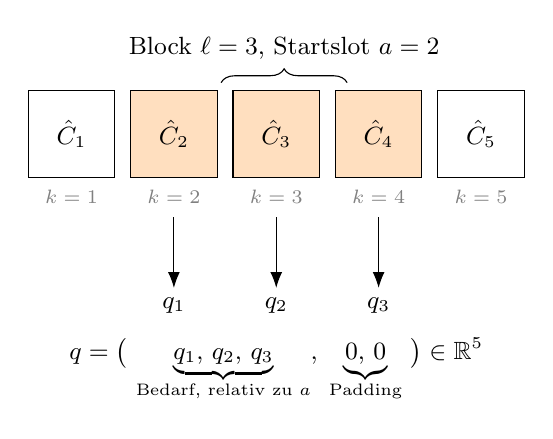
\begin{tikzpicture}[font=\small,
      slot/.style={draw, minimum width=11mm, minimum height=11mm},
      occ/.style ={draw, fill=orange!25, minimum width=11mm, minimum height=11mm},
      >={Latex[length=2mm]}
    ]
    % Slots 1..5, Slots 2-4 durch die Anfrage belegt (a=2, l=3)
    \node[slot] (s1) at (0,0) {$\hat C_1$};
    \node[occ]  (s2) at (1.3,0) {$\hat C_2$};
    \node[occ]  (s3) at (2.6,0) {$\hat C_3$};
    \node[occ]  (s4) at (3.9,0) {$\hat C_4$};
    \node[slot] (s5) at (5.2,0) {$\hat C_5$};

    \node[below=1pt, gray] at (s1.south) {\scriptsize $k=1$};
    \node[below=1pt, gray] at (s2.south) {\scriptsize $k=2$};
    \node[below=1pt, gray] at (s3.south) {\scriptsize $k=3$};
    \node[below=1pt, gray] at (s4.south) {\scriptsize $k=4$};
    \node[below=1pt, gray] at (s5.south) {\scriptsize $k=5$};

    % Block-Klammer über den belegten Slots
    \draw[decorate, decoration={brace, amplitude=5pt}] (1.85+0.05,0.65) -- (3.55-0.05,0.65)
      node[midway, above=5pt] {Block $\ell=3$, Startslot $a=2$};

    % q_i Zuordnung -- Pfeile starten unterhalb der k-Beschriftung, damit nichts überlappt
    \draw[->] (s2.south) ++(0,-0.5) -- ++(0,-0.9) node[below] {$q_1$};
    \draw[->] (s3.south) ++(0,-0.5) -- ++(0,-0.9) node[below] {$q_2$};
    \draw[->] (s4.south) ++(0,-0.5) -- ++(0,-0.9) node[below] {$q_3$};

    % Roher, gepolsterter Bedarfsvektor der Anfrage
    \node at (2.6,-3.0)
      {$q = \big(\, \underbrace{q_1,\,q_2,\,q_3}_{\text{Bedarf, relativ zu } a},\;
                    \underbrace{0,\,0}_{\text{Padding}} \,\big) \in \mathbb{R}^5$};
  \end{tikzpicture}
  \caption{Zustandsaufbau bei $K=5$ Slots und einer Anfrage der Länge $\ell=3$: Der Bedarfsvektor
    $q$ ist relativ zum (von der Aktion bestimmten) Startslot indiziert und mit $K-\ell=2$ Nullen
    auf feste Länge~$K$ aufgefüllt. Erst die gewählte Aktion $a$ ordnet $q_1,q_2,q_3$ den
    absoluten Slots $\hat C_2,\hat C_3,\hat C_4$ zu.}
  \label{fig:state-padding}
\end{figure}

\textbf{Konsequenz für die Monotonie.} Die hinteren $K-\ell$ Einträge von $q$ sind stets $0$ --
der kleinste Wert im kalibrierten Wertebereich von $q_k$. Das ist inhaltlich konsistent mit der
in Abschnitt~\ref{subsec:monotonicity} postulierten DECREASING-Monotonie: Ein Padding-Eintrag
bedeutet "kein Bedarf an dieser relativen Position" und wirkt im kalibrierten Modell wie eine
Anfrage ohne jede Einschränkung an diesem Slot -- was korrekt ist, da dieser Slot vom Block der
aktuellen Anfrage gar nicht betroffen ist.

\section{Monotonicity}
\label{sec:monotonicity}


\section{Experiments}
\label{sec:experiments}

\subsection{Setting}
\label{subsec:exp-setting}

For each \acs{drausp} benchmark instance, which are also used in the experiments of \textcite{drausp_lion18}, we train both the Standard-DQN baseline from
Section~\ref{sec:rl-approach} and the Lattice-DQN from Section~\ref{subsec:lattice-architecture}
using action masking, the target-network soft update, and the reject-biased $\epsilon$-greedy
exploration described earlier. To provide a fair comparision between the two networks, we adapt the layer sizes of the Standard-DQN to have the same number of parameters as the Lattice-DQN for each instance. 

\textbf{Parameters.} Unless noted otherwise, both networks are trained with the same
training-scheme parameters: reject-bias $\alpha=0.75$, $\gamma = 0.99$, $\epsilon$ decaying from
$1.0$ to $0.05$ over $T_d \cdot 1{.}000$ steps ($10{.}000$ for $T_d=10$, $20{.}000$ for $T_d=20$
and $50{.}000$ for $T_d=50$), a replay buffer of $50{.}000$ transitions with a $500$-step warm-up,
batch size $64$ and one training step every $4$ environment steps.

\textbf{Monotonicity test.} We evaluate the agents' monotonicity behavior every $100$ training
episodes by sampling $5$ trajectories, creating pairs of states as described in
Section~\ref{subsec:monotonicity-test}, and counting the number of monotonicity violations in
these pairs. This test is applied identically to both networks.

\textbf{Evaluation.} After performing $10{,}000$ training episodes, the agent's performance is evaluated; note that the network
weights do not change anymore here. We report the average performance on $10{,}000$ episodes with
$\epsilon = 0$. Monotonicity is evaluated by running the monotonicity tests for the different
parameters, each with $10{,}000$ pairs.

\textbf{Model comparison.} In Section~\ref{subsec:lattice-params} we determined the exact number
of parameters for the Lattice-DQN architecture dependent on the number of resources $K$,
calibrator keypoints $P$, and ensemble widths $U_1$ and $U_2$. We fix the number of calibrator keypoints $P=8$ and
the ensemble widths $U_1=4, U_2=2$, hence the number of parameters is only dependent on the number of resources
$K$. To obtain a fair comparison, we adapt the layer sizes of a two layer Standard-DQN to have the same
number of learnable parameters as the Lattice-DQN for each instance. We want to ensure by this that the model complexity is the same for both networks.


\subsection{Standard-DQN}
\label{subsec:exp-standard-dqn}

The Standard-DQN baseline is a standard two-layer feedforward network with no structural knowledge
of the monotonicity relations from Section~\ref{subsec:monotonicity}.

\textbf{Monotonicity behavior.} The standard DQN still manages to learn a policy that is mostly monotone, with only a few violations. Especially
the monotonicity in $C_k$ and the monotonicity in the mixed pairs is learned very well, and is fulfilled after few training episodes already.
Monotonicity in $t$ shows an interesting behavior: first the monotonicity drops to a ratio of $0.2$,
however during training the monotonicity recovers and gets to a perfect ratio of $1.0$ at the end. This behaviour can
be seen across different instances. 
The monotonicity in $q$ and $r$ is learned well from the beginning on and achieves a ratio $>0.8$ in the end. \\
An illustrative example of the training phase together with the monotonicity behavior is shown in Figure~\ref{fig:standard_dqn_training} for the benchmark instance SB05 with $T_d=50$.

\textbf{Performance.} After $4000$ episodes of training the agent's performance is already 
very good and a stable reward niveau is achieved. From this point on, the reward only increases slow and 
the $50$-episodes moving average fluctuates around the final reward.
The final evaluation phase shows that the agent achieves a very good performance, which is close to the optimal expected objective value $Z^*$ of the SDP formulation of \textcite{drausp_lion18}.
Remark that the result in the final evaluation is higher than in the training phase, which is due to the fact that the evaluation is performed with $\epsilon=0$ and therefore no random actions are taken.
\begin{figure}[ht]
	\centering
	\hspace*{-1.8cm}
	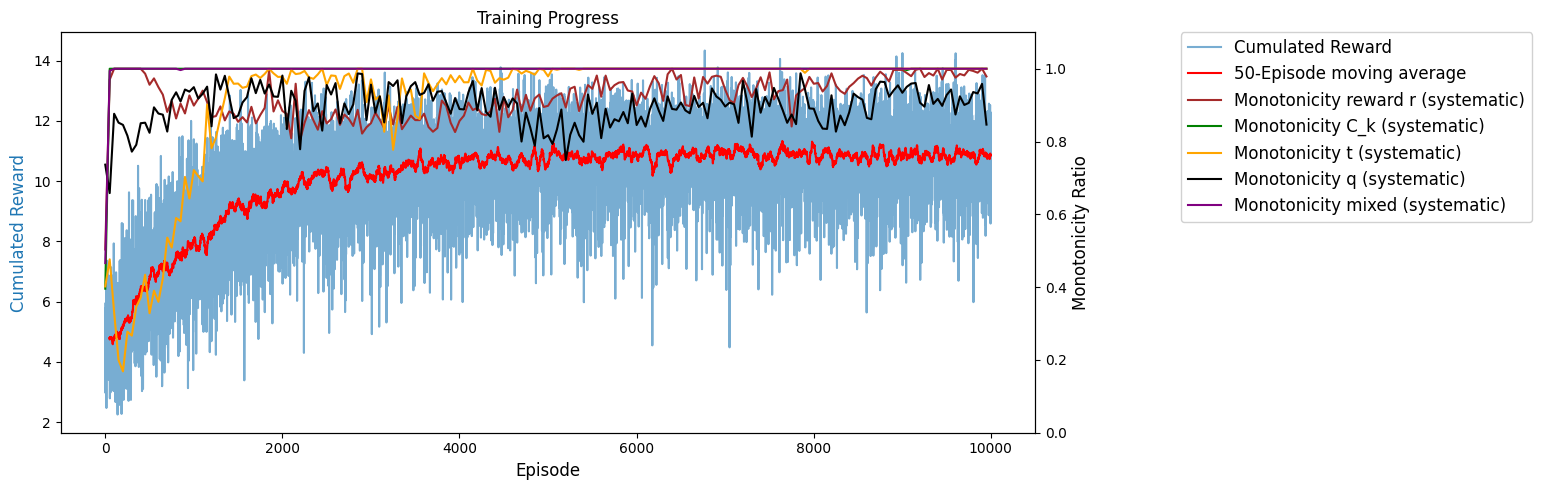
\includegraphics[scale=0.5]{grafiken/Experiments/standard_DQN_mono_SB5_all.png}
	\caption[Standard-DQN training and monotonicity behavior (SB05, $T_d=50$)]{Standard-DQN: training performance and monotonicity behavior on SB05, $T_d = 50$, over $10\,000$ training episodes.}
	\label{fig:standard_dqn_training}
\end{figure}
\begin{figure}[ht]
	\centering
	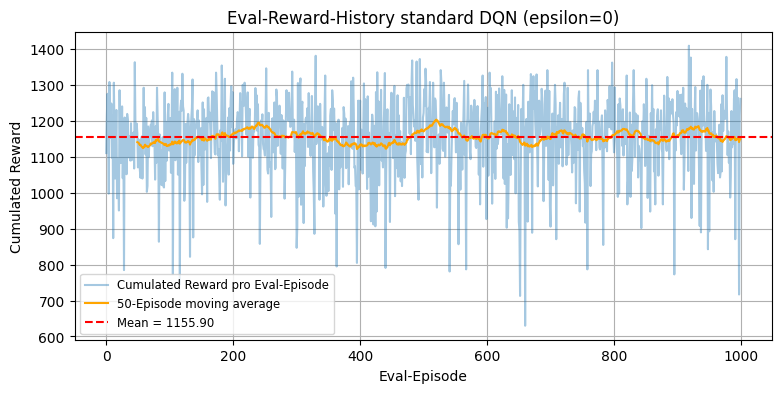
\includegraphics[scale=0.5]{grafiken/Experiments/standard_DQN_eval_SB5.png}
	\caption[Standard-DQN evaluation phase (SB05, $T_d=50$)]{Standard-DQN: evaluation phase on SB05, $T_d = 50$.}
	\label{fig:standard_dqn_eval}
\end{figure}

\subsection{Lattice-DQN}
\label{subsec:exp-lattice-dqn}

The Lattice-DQN is built up exactly as described in Section~\ref{subsec:lattice-architecture}.

\textbf{Monotonicity behavior.} Not surprisingly the monotonicity behavior is perfect from the
beginning on, as the network architecture enforces monotonicity by design. An example of the
training phase is shown in Figure~\ref{fig:lattice_dqn_training} for the benchmark instance SB05
with $T_d=50$.

\textbf{Performance.} Compared to a Standard-DQN with the same number of parameters, the agent has
to learn the same policy with a more constrained function class. This has to be taken into account
when designing the training architecture: the Lattice network needs considerably more fine-tuning
of the hyperparameters, whereas the Standard-DQN is much more robust to small changes in the
training-scheme hyperparameters (e.g.\ $\epsilon$-decay steps, reject bias, number of episodes).
Nevertheless, using the described training architecture in \ref{subsec:exp-setting}, the results are comparable
to the ones obtained by the standard \ac{dqn}. 

\begin{figure}[ht]
	\centering
	\hspace*{-1.8cm}
	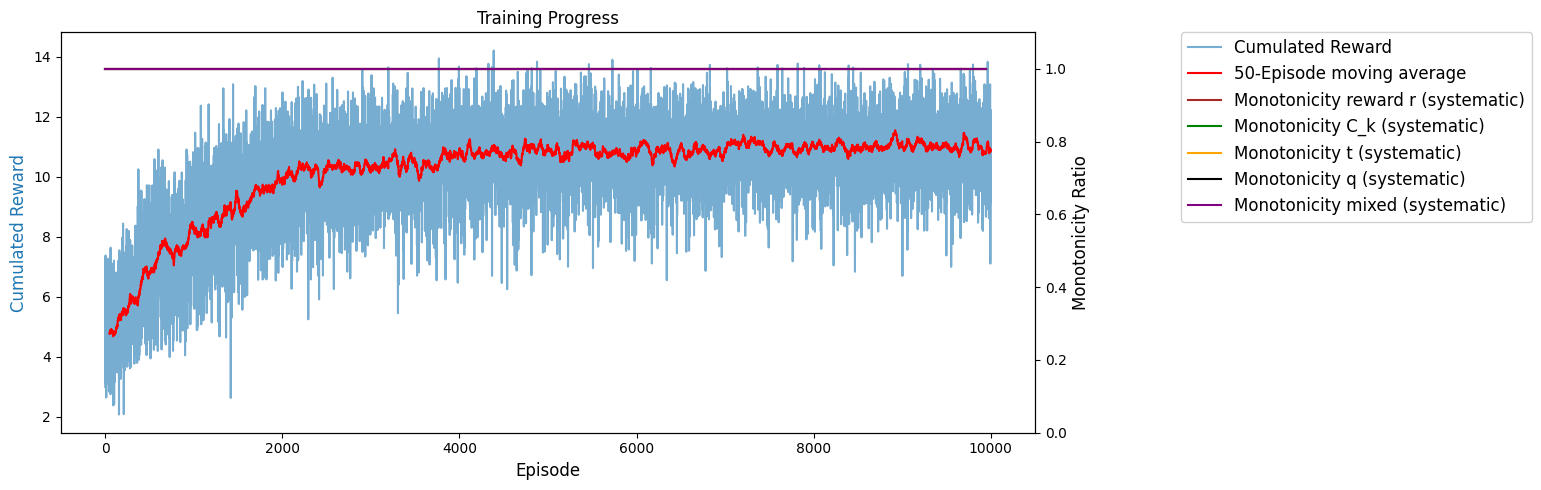
\includegraphics[scale=0.5]{grafiken/Experiments/Deep_Lattice_mono_SB5_all.png}
	\caption[Lattice-DQN training and monotonicity behavior (SB05, $T_d=50$)]{Lattice-DQN: training performance and monotonicity behavior on SB05, $T_d = 50$, over $10\,000$ training episodes.}
	\label{fig:lattice_dqn_training}
\end{figure}

\subsection{Numerical results}
\label{subsec:exp-results}

Tables~\ref{tab:results-s} and~\ref{tab:results-w} compare both agents against the optimal
expected objective value $Z^*$ of the SDP formulation of \textcite{drausp_lion18} (Table~1
and Table~2, respectively). $\bar R_{\text{eval}}$ is the mean cumulated reward over $10\,000$
evaluation episodes with $\epsilon = 0$, reported as mean $\pm$ one standard deviation across
those episodes. The monotonicity columns report the final ratio of
satisfied pairs ($10\,000$ pairs per axis) for the Standard-DQN; the Lattice-DQN satisfies every
check exactly by construction (ratio $1.00$ throughout) and is therefore omitted there. The
runtime columns are wall-clock seconds for the $10\,000$ training episodes and the $10\,000$
evaluation episodes, given as Standard-DQN\,/\,Lattice-DQN; entries marked $\dagger$ were
distorted by concurrent load on the shared machine and are not representative.

\begin{table}[htbp]
  \centering
  \footnotesize
  \setlength{\tabcolsep}{4pt}
  \caption[Results on the \texttt{lion18s} scheduling instances]{Results for the \texttt{lion18s} instances that require scheduling
    ($\text{len}(q) < K$; blocks \texttt{SA} $K=4$, \texttt{SB} $K=8$, \texttt{SC} $K=12$).
    $Z^*$ from \textcite{drausp_lion18}, Table~2.}
  \label{tab:results-s}
  \resizebox{\ifdim\width>\linewidth\linewidth\else\width\fi}{!}{%
  \begin{tabular}{l r r r r r r r r r r r}
    \toprule
     & & & \multicolumn{2}{c}{$\bar R_{\text{eval}} \pm s$} & \multicolumn{5}{c}{Monotonicity (Standard-DQN)} & \multicolumn{2}{c}{Runtime [s]} \\
    \cmidrule(lr){4-5}\cmidrule(lr){6-10}\cmidrule(lr){11-12}
    Instance & $T_d$ & $Z^*$ & DQN & Lat. & $C_k$ & $t$ & $r$ & $q_k$ & mix & train & eval \\
    \midrule
    SA01 & 10 & 5.08 & $5.08{\scriptstyle\,\pm\,0.85}$ & $5.03{\scriptstyle\,\pm\,0.86}$ & 0.99 & 1.00 & 0.90 & 0.84 & 1.00 & 266\,/\,2123 & 20\,/\,158 \\
    SA02 & 20 & 8.80 & $8.58{\scriptstyle\,\pm\,1.11}$ & $8.17{\scriptstyle\,\pm\,1.19}$ & 1.00 & 1.00 & 0.86 & 0.77 & 1.00 & 490\,/\,3387 & 39\,/\,295 \\
    SA03 & 50 & 13.44 & $13.10{\scriptstyle\,\pm\,1.10}$ & $12.39{\scriptstyle\,\pm\,1.03}$ & 1.00 & 0.74 & 0.82 & 0.84 & 1.00 & 1105\,/\,7403 & 92\,/\,1106 \\
    SA04 & 10 & 4.35 & $4.23{\scriptstyle\,\pm\,0.86}$ & $4.04{\scriptstyle\,\pm\,0.81}$ & 0.99 & 1.00 & 0.87 & 0.78 & 1.00 & 238\,/\,2494 & 19\,/\,262 \\
    SA05 & 20 & 5.97 & $5.87{\scriptstyle\,\pm\,0.69}$ & $4.49{\scriptstyle\,\pm\,0.79}$ & 1.00 & 0.96 & 0.82 & 0.80 & 1.00 & 447\,/\,3746 & 35\,/\,298 \\
    SA06 & 50 & 7.80 & $7.62{\scriptstyle\,\pm\,0.58}$ & $6.97{\scriptstyle\,\pm\,0.63}$ & 1.00 & 0.81 & 0.87 & 0.86 & 1.00 & 919\,/\,7374 & 78\,/\,802 \\
    SA07 & 10 & 5.08 & $5.06{\scriptstyle\,\pm\,0.85}$ & $5.09{\scriptstyle\,\pm\,0.84}$ & 1.00 & 1.00 & 0.96 & 0.77 & 1.00 & 255\,/\,39766$^{\dagger}$ & 20\,/\,269 \\
    SA08 & 20 & 10.16 & $10.16{\scriptstyle\,\pm\,1.18}$ & $10.08{\scriptstyle\,\pm\,1.23}$ & 1.00 & 1.00 & 0.91 & 0.83 & 1.00 & 539\,/\,4502 & 40\,/\,269 \\
    SA09 & 50 & 20.38 & $19.40{\scriptstyle\,\pm\,1.59}$ & $15.58{\scriptstyle\,\pm\,1.88}$ & 1.00 & 1.00 & 0.93 & 0.90 & 1.00 & 1214\,/\,7282 & 92\,/\,496 \\
    SA10 & 10 & 5.08 & $5.07{\scriptstyle\,\pm\,0.84}$ & $5.08{\scriptstyle\,\pm\,0.84}$ & 0.99 & 1.00 & 0.94 & 0.60 & 1.00 & 252\,/\,1825 & 21\,/\,138 \\
    SA11 & 20 & 9.02 & $8.47{\scriptstyle\,\pm\,1.03}$ & $8.17{\scriptstyle\,\pm\,1.25}$ & 1.00 & 1.00 & 0.87 & 0.77 & 1.00 & 490\,/\,3314 & 37\,/\,262 \\
    SA12 & 50 & 13.43 & $12.87{\scriptstyle\,\pm\,1.35}$ & $10.03{\scriptstyle\,\pm\,1.07}$ & 1.00 & 1.00 & 0.92 & 0.82 & 1.00 & 1102\,/\,6100 & 92\,/\,355 \\
    SA13 & 10 & 4.90 & $4.90{\scriptstyle\,\pm\,0.91}$ & $4.90{\scriptstyle\,\pm\,0.90}$ & 0.99 & 1.00 & 0.90 & 0.79 & 1.00 & 268\,/\,1818 & 20\,/\,134 \\
    SA14 & 20 & 8.79 & $8.55{\scriptstyle\,\pm\,1.12}$ & $8.27{\scriptstyle\,\pm\,1.24}$ & 1.00 & 1.00 & 0.96 & 0.80 & 1.00 & 494\,/\,3445 & 38\,/\,262 \\
    \addlinespace
    SB01 & 10 & 5.08 & $5.09{\scriptstyle\,\pm\,0.83}$ & $5.08{\scriptstyle\,\pm\,0.85}$ & 0.99 & 0.99 & 0.99 & 0.88 & 1.00 & 269\,/\,2672 & 21\,/\,289 \\
    SB02 & 20 & 10.16 & $10.04{\scriptstyle\,\pm\,1.23}$ & $10.03{\scriptstyle\,\pm\,1.23}$ & 0.98 & 1.00 & 0.96 & 0.88 & 1.00 & 543\,/\,65769$^{\dagger}$ & 42\,/\,4505$^{\dagger}$ \\
    SB03 & 10 & 5.08 & $5.03{\scriptstyle\,\pm\,0.87}$ & $5.03{\scriptstyle\,\pm\,0.87}$ & 0.99 & 1.00 & 0.87 & 0.87 & 1.00 & 269\,/\,2508 & 21\,/\,170 \\
    SB04 & 20 & 8.76 & $8.48{\scriptstyle\,\pm\,1.12}$ & $8.15{\scriptstyle\,\pm\,1.16}$ & 1.00 & 1.00 & 0.95 & 0.95 & 1.00 & 520\,/\,4655 & 39\,/\,329 \\
    SB05 & 50 & 12.60 & $12.05{\scriptstyle\,\pm\,0.87}$ & $7.77{\scriptstyle\,\pm\,1.49}$ & 1.00 & 0.96 & 0.88 & 0.85 & 1.00 & 1146\,/\,8399 & 92\,/\,474 \\
    SB06 & 10 & 4.44 & $4.25{\scriptstyle\,\pm\,0.73}$ & $4.15{\scriptstyle\,\pm\,0.76}$ & 1.00 & 0.99 & 0.81 & 0.81 & 1.00 & 252\,/\,2416 & 19\,/\,154 \\
    SB07 & 20 & 5.85 & $5.55{\scriptstyle\,\pm\,0.67}$ & $5.14{\scriptstyle\,\pm\,0.74}$ & 1.00 & 0.99 & 0.85 & 0.85 & 1.00 & 452\,/\,4223 & 35\,/\,254 \\
    SB08 & 50 & 7.53 & $7.00{\scriptstyle\,\pm\,0.55}$ & $6.18{\scriptstyle\,\pm\,0.81}$ & 1.00 & 0.62 & 0.85 & 0.78 & 1.00 & 966\,/\,8246 & 73\,/\,489 \\
    SB09 & 10 & 3.38 & $3.24{\scriptstyle\,\pm\,0.58}$ & $3.21{\scriptstyle\,\pm\,0.59}$ & 0.98 & 0.99 & 0.83 & 0.93 & 1.00 & 253\,/\,2552 & 20\,/\,163 \\
    SB10 & 20 & 4.28 & $3.90{\scriptstyle\,\pm\,0.52}$ & $4.02{\scriptstyle\,\pm\,0.54}$ & 0.98 & 0.95 & 0.87 & 0.85 & 1.00 & 487\,/\,4678 & 35\,/\,308 \\
    \addlinespace
    SC01 &  5 & 2.54 & $2.50{\scriptstyle\,\pm\,0.60}$ & $2.50{\scriptstyle\,\pm\,0.60}$ & 0.99 & 1.00 & 0.98 & 0.90 & 1.00 & 141\,/\,1659 & 11\,/\,94 \\
    SC02 &  5 & 2.32 & $2.22{\scriptstyle\,\pm\,0.57}$ & $2.23{\scriptstyle\,\pm\,0.58}$ & 0.98 & 0.98 & 0.96 & 0.74 & 1.00 & 141\,/\,1615 & 11\,/\,89 \\
    SC03 &  5 & 1.74 & $1.68{\scriptstyle\,\pm\,0.40}$ & $1.61{\scriptstyle\,\pm\,0.40}$ & 0.98 & 0.97 & 0.86 & 0.87 & 1.00 & 126\,/\,1454 & 9\,/\,80 \\
    SC04 & 10 & 2.17 & $2.04{\scriptstyle\,\pm\,0.37}$ & $2.06{\scriptstyle\,\pm\,0.38}$ & 0.99 & 0.97 & 0.91 & 0.91 & 1.00 & 225\,/\,2648 & 16\,/\,154 \\
    SC05 & 20 & 2.55 & $2.40{\scriptstyle\,\pm\,0.31}$ & $2.29{\scriptstyle\,\pm\,0.35}$ & 0.97 & 0.94 & 0.89 & 0.82 & 1.00 & 412\,/\,4365 & 30\,/\,264 \\
    \bottomrule
  \end{tabular}%
  }
\end{table}

\begin{table}[htbp]
  \centering
  \footnotesize
  \setlength{\tabcolsep}{4pt}
  \caption[Results on the \texttt{lion18w} accept/reject instances]{Results for the \texttt{W} instances (\texttt{lion18w}; blocks \texttt{WA} $K=4$,
    \texttt{WB} $K=8$, \texttt{WC} $K=12$, all with $\text{len}(q) = K$, i.e.\ accept/reject only).
    $Z^*$ from \textcite{drausp_lion18}, Table~1.}
  \label{tab:results-w}
  \resizebox{\ifdim\width>\linewidth\linewidth\else\width\fi}{!}{%
  \begin{tabular}{l r r r r r r r r r r r}
    \toprule
     & & & \multicolumn{2}{c}{$\bar R_{\text{eval}} \pm s$} & \multicolumn{5}{c}{Monotonicity (Standard-DQN)} & \multicolumn{2}{c}{Runtime [s]} \\
    \cmidrule(lr){4-5}\cmidrule(lr){6-10}\cmidrule(lr){11-12}
    Instance & $T_d$ & $Z^*$ & DQN & Lat. & $C_k$ & $t$ & $r$ & $q_k$ & mix & train & eval \\
    \midrule
    WA01 & 10 & 4.33 & $4.25{\scriptstyle\,\pm\,0.84}$ & $4.13{\scriptstyle\,\pm\,0.87}$ & 0.99 & 1.00 & 0.82 & 0.62 & 1.00 & 244\,/\,1900 & 19\,/\,153 \\
    WA02 & 20 & 6.43 & $6.11{\scriptstyle\,\pm\,0.99}$ & $5.81{\scriptstyle\,\pm\,1.04}$ & 0.99 & 0.98 & 0.65 & 0.78 & 1.00 & 457\,/\,3181 & 37\,/\,268 \\
    WA03 & 50 & 9.49 & $8.65{\scriptstyle\,\pm\,1.14}$ & $7.78{\scriptstyle\,\pm\,1.48}$ & 1.00 & 0.98 & 0.73 & 0.60 & 1.00 & 1046\,/\,5694 & 91\,/\,564 \\
    WA04 & 10 & 5.07 & $5.08{\scriptstyle\,\pm\,0.84}$ & $5.07{\scriptstyle\,\pm\,0.85}$ & 1.00 & 1.00 & 0.79 & 0.52 & 1.00 & 250\,/\,1962 & 20\,/\,167 \\
    WA05 & 20 & 9.23 & $9.09{\scriptstyle\,\pm\,1.20}$ & $8.24{\scriptstyle\,\pm\,1.60}$ & 1.00 & 1.00 & 0.79 & 0.64 & 1.00 & 491\,/\,3385 & 38\,/\,284 \\
    WA06 & 50 & 15.36 & $14.44{\scriptstyle\,\pm\,1.43}$ & $9.07{\scriptstyle\,\pm\,1.83}$ & 1.00 & 0.99 & 0.84 & 0.75 & 1.00 & 1144\,/\,5649 & 90\,/\,320 \\
    WA07 & 10 & 4.35 & $4.29{\scriptstyle\,\pm\,0.88}$ & $3.99{\scriptstyle\,\pm\,0.99}$ & 0.98 & 1.00 & 0.85 & 0.60 & 1.00 & 247\,/\,1766 & 19\,/\,144 \\
    WA08 & 20 & 6.58 & $6.35{\scriptstyle\,\pm\,1.05}$ & $5.58{\scriptstyle\,\pm\,1.23}$ & 1.00 & 0.99 & 0.83 & 0.73 & 1.00 & 460\,/\,3179 & 37\,/\,250 \\
    \addlinespace
    WB01 & 10 & 4.08 & $3.94{\scriptstyle\,\pm\,0.74}$ & $3.89{\scriptstyle\,\pm\,0.76}$ & 0.99 & 1.00 & 0.84 & 0.70 & 1.00 & 242\,/\,2346 & 18\,/\,151 \\
    WB02 & 20 & 5.47 & $5.08{\scriptstyle\,\pm\,0.71}$ & $4.90{\scriptstyle\,\pm\,0.78}$ & 0.99 & 0.98 & 0.75 & 0.75 & 1.00 & 440\,/\,3946 & 34\,/\,250 \\
    WB03 & 50 & 7.19 & $6.69{\scriptstyle\,\pm\,0.73}$ & $5.68{\scriptstyle\,\pm\,0.82}$ & 1.00 & 0.99 & 0.81 & 0.86 & 1.00 & 891\,/\,6760 & 83\,/\,489 \\
    WB04 & 10 & 1.69 & $1.67{\scriptstyle\,\pm\,0.43}$ & $1.66{\scriptstyle\,\pm\,0.42}$ & 0.97 & 0.96 & 0.69 & 0.77 & 1.00 & 215\,/\,2140 & 18\,/\,147 \\
    WB05 & 20 & 2.08 & $2.01{\scriptstyle\,\pm\,0.43}$ & $1.93{\scriptstyle\,\pm\,0.44}$ & 0.98 & 0.96 & 0.69 & 0.72 & 1.00 & 434\,/\,3767 & 31\,/\,248 \\
    WB06 & 10 & 3.22 & $3.17{\scriptstyle\,\pm\,0.59}$ & $3.11{\scriptstyle\,\pm\,0.61}$ & 0.98 & 0.99 & 0.86 & 0.74 & 1.00 & 239\,/\,2335 & 19\,/\,160 \\
    WB07 & 20 & 4.06 & $3.94{\scriptstyle\,\pm\,0.57}$ & $3.58{\scriptstyle\,\pm\,0.59}$ & 0.98 & 0.99 & 0.72 & 0.80 & 1.00 & 460\,/\,4480 & 35\,/\,248 \\
    \addlinespace
    WC01 & 10 & 1.54 & $1.52{\scriptstyle\,\pm\,0.30}$ & $1.48{\scriptstyle\,\pm\,0.29}$ & 0.99 & 0.95 & 0.79 & 0.79 & 0.99 & 223\,/\,2629 & 17\,/\,139 \\
    WC02 & 20 & 1.78 & $1.75{\scriptstyle\,\pm\,0.28}$ & $1.71{\scriptstyle\,\pm\,0.25}$ & 1.00 & 0.96 & 0.72 & 0.69 & 0.96 & 400\,/\,4663 & 30\,/\,245 \\
    WC03 & 50 & 2.13 & $2.02{\scriptstyle\,\pm\,0.30}$ & $1.60{\scriptstyle\,\pm\,0.31}$ & 1.00 & 0.90 & 0.82 & 0.46 & 0.98 & 851\,/\,9007 & 64\,/\,405 \\
    WC04 & 10 & 1.53 & $1.52{\scriptstyle\,\pm\,0.35}$ & $1.48{\scriptstyle\,\pm\,0.35}$ & 0.99 & 0.96 & 0.65 & 0.57 & 0.99 & 228\,/\,2670 & 17\,/\,146 \\
    WC05 & 20 & 1.79 & $1.73{\scriptstyle\,\pm\,0.30}$ & $1.72{\scriptstyle\,\pm\,0.30}$ & 0.98 & 0.95 & 0.82 & 0.91 & 1.00 & 412\,/\,4560 & 29\,/\,271 \\
    WC06 & 50 & 2.17 & $1.92{\scriptstyle\,\pm\,0.34}$ & $1.88{\scriptstyle\,\pm\,0.32}$ & 1.00 & 0.78 & 0.38 & 0.66 & 1.00 & 890\,/\,8836 & 58\,/\,483 \\
    \bottomrule
  \end{tabular}%
  }
\end{table}

The Standard-DQN reaches $90$--$100\%$ of $Z^*$ on almost all instances and is at or above the
Lattice-DQN in evaluation reward essentially everywhere. The Lattice-DQN matches it on the easy
instances but falls off markedly on the harder large-$T_d$ cases, where its more constrained
function class limits the attainable policy: e.g.\ SB05 ($7.77$ vs.\ $12.05$, $62\%$ of $Z^*$),
SA09 ($15.58$ vs.\ $19.40$), WA06 ($9.07$ vs.\ $14.44$) and WC03 ($1.60$ vs.\ $2.02$). The
Standard-DQN learns monotonicity in $C_k$, $t$ and the mixed pairs almost perfectly, but only
partially in $r$ and especially $q_k$, which drops below $0.6$ on some instances (SA10, WA04,
WC03). Training the Lattice-DQN takes roughly $5$--$12\times$ longer than the parameter-matched
Standard-DQN, caused by the per-step constraint projection and the many small lattice
evaluations.

\section{Conclusion}
\label{sec:conclusion}

We developed a representation of the \acs{drausp} as a finite-horizon \acs{mdp}, which enables us
to use reinforcement learning techniques to learn acceptance and scheduling policies. For optimization, we used
a value-based deep \acs{rl} approach, specifically Q-learning with a deep neural network as function approximator.
We constructed a stable baseline approach in Section \ref{sec:rl-approach} using a Standard \acs{dqn}. We
tested the behaviour of the learned $Q$-function with respect to monotonicity relations inherent to the problem.
Doing so, we constructed a monotonicity test to evaluate the learned $Q$-function (see \ref{subsec:monotonicity-test}).\\
As a second approach, we took advantage of the known monotonicity relations presented in \ref{subsec:monotonicity} 
and constructed a monotonicity-aware \acs{dqn}, using lattice layers. We built up a deep lattice
network architecture that enforces monotonicity by design, and again evaluated its performance 
and monotonicity behaviour on the same benchmark instances as the Standard \acs{dqn}.\\
We saw that even without any knowledge about the problem structure at the beginning, the
Standard \acs{dqn} still manages to learn monotonicity. The Lattice-\acs{dqn} 
on the other hand, enforces monotonicity by design and therefore satisfies all monotonicity tests exactly. 
But using the Lattice-\acs{dqn} comes with a trade-off: the more constrained function class of the Lattice-\acs{dqn}
makes it harder to learn the optimal policy. This leads to a slower convergence and a slightly worse performance in the end.\\

Future work could focus on improving the performance of the Lattice-\acs{dqn} by using a more complex architecture, e.g. by
adding more layers or increasing the number of lattices per layer. Another approach could be to enforce monotonicity only on a subset of the features.
In this case one could use a hybrid architecture,
where non-monotonic features are first processed by standard feedforward layers, while the monotonicity-relevant features
bypass these layers (or only pass through monotone transformations) and are combined with the resulting representation only
at the final lattice layers. This would allow the network to learn a more complex function from the non-monotonic features
while still enforcing end-to-end monotonicity with respect to the relevant inputs. Note that simply stacking feedforward
layers before lattice layers on all inputs would not preserve this guarantee, since composing a monotone function with a
non-monotone one is generally not monotone.
In our numerical experiments the Standard \acs{dqn} still manages to learn monotonicity, but it is not guaranteed to do so.
One could test if this holds true if the network architecture is changed or instances get larger and more complex.

\clearpage
\printbibliography
\addcontentsline{toc}{section}{References}

\clearpage
\section*{Eidesstattliche Erklärung}

Ich erkläre hiermit an Eides statt, dass ich die vorliegende Arbeit
ohne Hilfe Dritter und ohne Benutzung anderer als der angegebenen
Hilfsmittel angefertigt habe; die aus fremden Quellen direkt oder
indirekt übernommenen Gedanken sind als solche kenntlich gemacht. Die
Arbeit wurde bisher in gleicher oder ähnlicher Form in keiner anderen
Prüfungsbehörde vorgelegt und auch noch nicht veröffentlicht.

\vspace{1in}

\par\noindent\makebox[2.0in]{\hrulefill} \hfill\makebox[2.5in]{\hrulefill}%
\par\noindent\makebox[2.0in][l]{Ort, Datum}      \hfill\makebox[2.5in][l]{Unterschrift}%
\end{document}
